\documentclass[11pt,letterpaper]{article}
\usepackage[margin=0.9in,headheight=14pt]{geometry}
\usepackage[T1]{fontenc}
\usepackage[utf8]{inputenc}
\usepackage{lmodern,microtype}
\usepackage{amsmath,amssymb,amsthm,mathtools}
\usepackage{booktabs,longtable,array,enumitem}
\usepackage{tikz}
\usetikzlibrary{arrows.meta,positioning,shapes.geometric,calc}
\usepackage{hyperref}
\usepackage{fancyhdr}
\hypersetup{colorlinks=false,pdfborder={0 0 0},pdfauthor={ChatGPT (OpenAI)},pdftitle={What Survives the Successor?}}
\urlstyle{same}
\setcounter{tocdepth}{1}
\setlength{\parskip}{4pt}
\setlength{\parindent}{12pt}
\raggedbottom
\emergencystretch=2em
\pagestyle{fancy}
\fancyhf{}
\fancyhead[L]{\small What Survives the Successor?}
\fancyhead[R]{\small Research synthesis 001}
\fancyfoot[C]{\thepage}
\newtheorem{theorem}{Theorem}[section]
\newtheorem{proposition}[theorem]{Proposition}
\newtheorem{corollary}[theorem]{Corollary}
\newtheorem{lemma}[theorem]{Lemma}
\theoremstyle{definition}
\newtheorem{definition}[theorem]{Definition}
\newtheorem{example}[theorem]{Example}
\newtheorem{counterexample}[theorem]{Counterexample}
\theoremstyle{remark}
\newtheorem{remark}[theorem]{Remark}
\newcommand{\K}{\mathcal K}
\newcommand{\F}{\mathcal F}
\newcommand{\Act}{\mathsf{Act}}
\newcommand{\Out}{\mathsf{Out}}
\newcommand{\Win}{\mathsf{Win}}
\newcommand{\View}{\mathsf{View}}
\newcommand{\Auth}{\mathsf{Auth}}
\newcommand{\Val}{\mathsf{Val}}
\newcommand{\Bank}{\mathsf{BANK}}
\newcommand{\prooflink}[1]{\hfill\hyperlink{proof:#1}{\footnotesize[proof in PROOFS]}}
\newcommand{\backlink}[1]{\hyperlink{claim:#1}{\footnotesize[back to statement]}}
\newcommand{\src}[1]{\textup{[#1]}}
\newcommand{\status}{\textsc{paper-level, not independently certified}}
\title{\bfseries What Survives the Successor?\\[4pt]
\large Certified Evidence, Adversarial Settlement, and the Costs of Changing a Theorem Prover}
\author{Research and writing: ChatGPT (OpenAI)\\[3pt]
\small Research Director: Brian Tenneson}
\date{November 16, 2026\\\small Tenneson1-style integrated theory manuscript --- research draft 001}
\begin{document}
\maketitle
\begin{center}\normalsize See the AI disclaimer that follows this essay.\end{center}
\begin{abstract}
An automated theorem prover can keep proving the same propositions and yet change which proofs it can obtain within a budget. That difference becomes harder to assess when the revision creates a distinct successor, transfers qualified evidence, and introduces nondeterministic execution. We begin with the formal-system, SIC, and ATP distinctions that make a revision a mathematical object, then reconstruct conservative derived-rule compilation and the role of a verifier-qualified ledger. Next we separate a change in mathematical consequences from a change in discovery access, and distinguish self-simulation from a distinct simulator's representation. Against that background we formulate an evidence-gated, one-sided \emph{alternating cost refinement}: under explicit authorization, observation, branch, and charge hypotheses, a successor can lift a predecessor's forced-settlement strategy without increasing its optimal worst-case per-episode cost. A checkable strict action advantage and a fully charged one-time overhead yield an amortized improvement theorem. A two-branch finite construction shows the exact evidence threshold and two-episode break-even point, while an imitation obstruction rules out strict superiority over a comparator with the same upgrade permissions. We then integrate coordinated basin escape and finite revision/completion dynamics, retaining counterexamples to global optimality, general discovery, and unbounded extrapolation. The resulting contribution is a source-grounded conditional synthesis, with new paper-level formulations and explicit proof obligations. No FORGE-6-E experiment, installed successor improvement, or independent proof-kernel check is claimed.
\end{abstract}
\noindent\textbf{Keywords:} semi-ideal computers; automated theorem proving; certified revision; epistemic handoff; alternating simulation; adversarial settlement; amortized cost; improvement basins; finite completion.
\tableofcontents

\section{The question is not whether the machine changed its name}
A proof about a machine is not the same as a modification to its executable. A modification may preserve every theorem and still alter the time needed to find one. A shorter route may increase charged resource use. A successfully simulated execution may conceal a nondeterministic branch that never reaches a certificate. An evidence-carrying successor may preserve a predecessor's valid mathematical claims without preserving the predecessor's identity. These are separations, not successive rhetorical descriptions of one event.

The twelve distinct works supplied for this investigation develop these distinctions from formal systems through proof-cache feedback, mathematical awareness, succession, economics, settlement navigation, escape basins and completion \src{1--12}. We neither merge equivalent theorems into spurious new results nor treat a second edition as independent evidence. The strongest new question here is therefore not whether a successor can be declared better, but whether \emph{usable evidence plus a fully branched, cost-aware refinement} can support an actual mathematical improvement statement.

We apply a stringent rule: the target and hypotheses are frozen before each argument; proof, code, evidence, branch coverage, and deployment economy occupy different verification gates. The original unrestricted ambition remains unresolved. The limited positive claims that follow are conditional mathematics, with human-readable arguments collected in the sole appendix \textbf{PROOFS}.

\begin{figure}[htbp]\centering
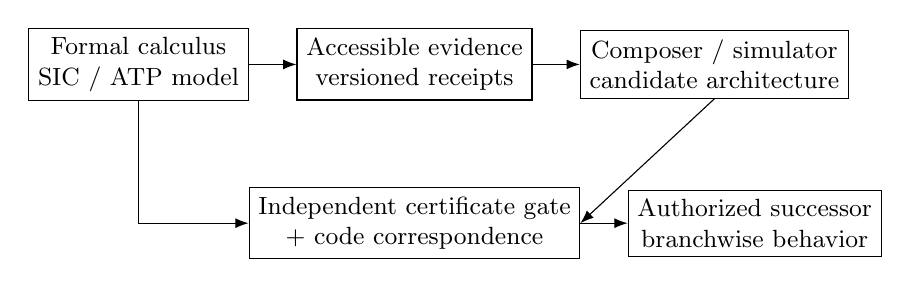
\begin{tikzpicture}[node distance=8mm and 6mm, every node/.style={font=\small}, >=Latex]
\node[draw,minimum width=2.8cm,align=center] (f) {Formal calculus\\SIC / ATP model};
\node[draw,right=of f,minimum width=2.8cm,align=center] (ev) {Accessible evidence\\versioned receipts};
\node[draw,right=of ev,minimum width=2.8cm,align=center] (co) {Composer / simulator\\candidate architecture};
\node[draw,below=11mm of ev,minimum width=3.2cm,align=center] (gate) {Independent certificate gate\\+ code correspondence};
\node[draw,right=of gate,minimum width=3.0cm,align=center] (q) {Authorized successor\\branchwise behavior};
\draw[->] (f)--(ev);\draw[->] (ev)--(co);\draw[->] (co.south)--(gate.east);
\draw[->] (gate)--(q);\draw[->] (f.south) |- (gate.west);
\end{tikzpicture}
\caption{Distinct obligations on the route from a theorem-proving object to a successor. The arrows represent required witnesses, not executed software interfaces.}\end{figure}

\section{Formal machines, representation, and the type of a revision}
The broad $xyz$ convention represents a formal system by $F=(x,y,z)$: an alphabet or symbol domain, a designated set of finite well-formed strings, and a family of inference operations. The set $y$ need not itself be generated by a recursive grammar; executability and structural induction need extra hypotheses \src{1}. A proof from $\Gamma$ is a finite derivation, and $\operatorname{Con}_F(\Gamma)$ collects its conclusions. This is more restrictive than membership in $y$.

A \emph{semi-ideal computer} (SIC) is a staged computational object satisfying the stipulated stage and halting conventions. An \emph{automated theorem prover} (ATP) is an SIC with additional theorem-proving obligations. An AMLD is a further architecture or protocol class, not a synonym for all SICs or ATPs. The supplied papers make the distinctions operationally important: a composer SIC may construct a revision; an ATP may derive its proof; a subject SIC may receive it; a simulator may predict its behavior; a trusted checker may authorize a mathematical claim. These roles may coincide or remain distinct \src{1,4,7}.

\begin{definition}[Frozen revision contract]\label{def:contract}
A contract $\K$ records $F,\Gamma$, exact target and accepted certificate language, verifier regime and version, initial $\Bank$ imports, permitted architectures and revisions, role assignments, scheduler and failure assumptions, branch ownership, observations and hidden information, workload, time horizon, all charge types and reuse rights, plus the authorized installation and handoff actions. A revision state is
\[
 X_n=(A_n,\pi_n,L_n,E_n,B_n,H_n),\qquad X_{n+1}\in\F_{\K}(X_n),
\]
where $L$ is the evidence/provenance ledger, $E$ the accessible witnesses, $B$ remaining spendable budget, and $H$ immutable history. The map $\F_{\K}$ may be partial, set-valued, or adversarial. Total charged expense is a separate coordinate from remaining budget and future per-episode objective.
\end{definition}

The distinction between representation, audit and certified update is the Picard feedback loop $P_{n+1}=\F(P_n)$ of the source framework \src{2,3}. Its epoch $n$ is different from a staged inference index and from a reflection-depth index. Formal self-awareness means a machine can derive statements concerning a designated formal name; it does not thereby prove facts about installed code, and it does not entail subjective experience. A checked code-to-description interpretation is required before operational inferences follow \src{3,6}.

\section{What the ledger is allowed to preserve}
Epistemic awareness in the supplied handoff framework is a typed relation among a subject, a proposition, an accessible record and a verifier. Its central question is not whether some proof exists, but whether the subject possesses a suitably scoped witness it may legitimately use. In particular, a receipt about the predecessor is not automatically a valid assertion about the successor, and a verifier change cannot be treated as a change in font \src{5}.

\begin{definition}[Qualified, successor-safe record]\label{def:record}
A record $r$ for proposition $\varphi$ is \emph{qualified} relative to $(\K,V)$ when $r\in\View(X)$, $V$ accepts its finite proof support under the frozen theory and scope, and its dependency, verifier-version and rights fields are valid. A handoff $h:P\rightsquigarrow Q$ is \emph{receipt-preserving} on a declared ledger class if, for every qualifying $r$, it supplies a translated or replayable record $h_*r\in\View(Q)$ accepted under the declared target verifier for the same semantically invariant claim and scope; provenance and issuer identity are recorded without identifying the two subjects.
\end{definition}

\begin{proposition}[Scoped knowledge transport, inherited]\label{prop:transport}\hypertarget{claim:transport}{}
A receipt-preserving handoff transports the authorized truth claim of every retained ledger entry, assuming both verifiers are sound on their declared domains and the proof interpretations agree on that entry. It need not preserve the original machine identity. \src{5, Lemma 6.3 and Corollary 6.4}\prooflink{transport}
\end{proposition}

This proposition has a deliberately narrow proof. Actual difficulty lies in establishing replay/translation and semantic invariance from concrete artifacts. No bytes-only copying claim may be admitted to $\Bank$ merely because the predecessor once accepted it.

\begin{counterexample}[Certificate bytes without assumptions]\label{cex:scope}\hypertarget{claim:scope}{}
The one-line certificate for $p$ under premises $\{p\}$ does not establish $p$ from an empty premise set. A successor that changes $\Gamma$ and copies the same proof string has changed the proposition's authorization context, not preserved it. This is the obstruction of \src{7, Prop. 5.2}.\prooflink{scope}
\end{counterexample}

\begin{figure}[htbp]\centering
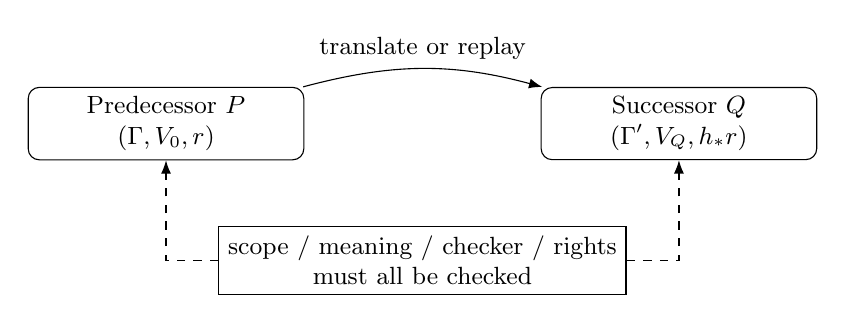
\begin{tikzpicture}[>=Latex,every node/.style={font=\small},node distance=13mm]
\node[draw,rounded corners,align=center,minimum width=3.5cm] (p) {Predecessor $P$\\$(\Gamma,V_0,r)$};
\node[draw,rounded corners,align=center,right=3.0cm of p,minimum width=3.5cm] (q) {Successor $Q$\\$(\Gamma',V_Q,h_*r)$};
\node[draw,align=center,below=of $(p)!0.5!(q)$] (g) {scope / meaning / checker / rights\\must all be checked};
\draw[->] (p) to[bend left=15] node[above]{translate or replay} (q);
\draw[dashed,->] (g.west) -| (p.south);\draw[dashed,->] (g.east) -| (q.south);
\end{tikzpicture}
\caption{Evidence transport preserves scoped mathematical content, not a magical equation of predecessor and successor identities.}\end{figure}

\section{Conservative change and the executable gap}
An immediately useful revision adds a rule $d$ that abbreviates a finite base-system derivation. If $d(a_1,\ldots,a_k)=b$ only when $\{a_1,\ldots,a_k\}\vdash_F b$, the enlarged calculus can replay each macro as an ordinary proof. This is the same expansion argument appearing in several sources \src{1--4,8}; it is one inherited result, not four independent discoveries.

\begin{theorem}[Conservative derived-rule compilation, inherited]\label{thm:conservative}\hypertarget{claim:conservative}{}
Let $F'$ retain all original rules of $F$ and add only $F$-derived rules, with sound, finitely replayable expansions. For every $\Gamma,\varphi$, 
\[
 \Gamma\vdash_{F'}\varphi\quad\Longleftrightarrow\quad\Gamma\vdash_F\varphi.
\]
This alone says nothing about executable implementation, charged cost, or the time of first discovery. \src{1, Thm. 10.2; 2, Thm. 5.3}\prooflink{conservative}
\end{theorem}

A wider architecture change might alter the proof-search schedule, stored dependencies, translated certificate syntax, nondeterministic continuations or complete program code. In that case a pure calculus-level argument is not enough. One also needs a separately checked relation linking the installed implementation to its declared semantics and proving that all permitted emitted results satisfy the accepted proof protocol. The accepted checker cannot simply certify its own new authority without a trusted meta-checker or explicit retained trusted basis.

\begin{proposition}[Safety and value are independent obligations]\label{prop:safety}\hypertarget{claim:safety}{}
A sound proof checker and a safe trace refinement do not imply forced termination or reduced cost. Likewise, a syntactically valid derived rule may increase fully charged processing cost when lookup, memory, or checking overhead exceeds the saved inference transitions.\prooflink{safety}
\end{proposition}

The proposition is not a pessimistic reservation: it tells us which further theorems a successor construction needs. The remainder of the paper equips the program with explicit branchwise forcing and a full cost comparison.

\section{Discovery versus a beneficial architecture}
The existence of a finite proof-carrying revision is a mathematical assertion. The ability to enumerate and check it is a second assertion. The economic superiority of adopting it is a third. The composer paper \src{4} separates these; the successor paper \src{7} adds verifier-compatible handoff and branch-rank witnesses.

\begin{theorem}[Finite-witness discoverability, inherited]\label{thm:enumerate}\hypertarget{claim:enumerate}{}
Let a class of finite candidate-and-certificate pairs be effectively enumerated, and let its acceptance predicate be total, sound and decidable on these finite encodings. If the class contains an accepted witness, fair enumeration eventually finds one. This algorithm does not decide that no witness exists in a potentially infinite class. \src{4, Thm. 6.1; 7, Thm. 3.2}\prooflink{enumerate}
\end{theorem}

For example, the three inference transitions $a\to b\to c\to d$ can be bundled into one certified derived rule $a\Rightarrow d$. On a declared workload of $N$ identical uses, a stipulated one-unit macro execution and $B$ units of \emph{complete} one-time investigation and installation charge give $3N$ versus $B+N$; saving occurs exactly when $2N>B$. This is a finite mathematical example from the source literature \src{7,8}. The first proof or macro may be expensive to discover, rejected proposals must be charged, and the source theorem does not claim that every competing adaptive prover requires three units per use.

\begin{theorem}[Charged break-even criterion]\label{thm:break}\hypertarget{claim:break}{}
Suppose a fixed workload has $N$ episodes, and on episode $i$ every permitted execution of the installed new policy costs at most $q_i$ while the best specified old-architecture adaptive policy costs at least $\ell_i$. If all one-time expenses are bounded by $B$, the new candidate has strictly smaller complete charged cost whenever
\[
       \sum_{i=1}^N(\ell_i-q_i)>B.
\]
For repeated identical bounds $\ell_i\geq L$, $q_i\leq q$, it suffices that $N(L-q)>B$. The inequality itself does not certify the correctness of either bound.\prooflink{break}
\end{theorem}

\section{The two simulation questions}
The source corpus explicitly separates a simulator $P$ from a simulated subject $S$. Self-simulation $P=S$ is a special type-correct case, not the definition of simulation. When a distinct simulator describes $S$, its observable behaviors must be connected through a witness; a mere formal name for $S$ does not establish predictive accuracy \src{4,7}. Under a clocked simulation, theoremhood or termination may transport while the number or cost of intermediate steps changes \src{10}.

\begin{definition}[Game semantics for a forced settlement]\label{def:game}
A finite reachability game $G=(X,T,\Act,\Out,c)$ has an accepting terminal set $T$, a finite set of controller actions $\Act(x)$ at each nonterminal state, nonempty adversarial successor sets $\Out(x,a)$, and nonnegative rational charges $c(x,a,y)$. Every terminal certificate must be accepted under the frozen proof and evidence contract. A controller \emph{forces settlement} if every admitted adversarial continuation under its observation-respecting policy reaches $T$. Define the minimum worst-case cost
\[
 V_G(x)=\inf_{\pi\ \mathrm{forcing}}\;\sup_{\omega\ \mathrm{admitted\ under}\ \pi}\;\sum_{e\in\omega}c(e),
\]
with value $+\infty$ when no forcing policy exists in the adequate declared game. In a finite decreasing-rank game this is calculated by
\[
 V_G(x)=\begin{cases}0&x\in T,\\
 \displaystyle\min_{a\in\Act(x)}\max_{y\in\Out(x,a)}\bigl(c(x,a,y)+V_G(y)\bigr)&x\notin T.
 \end{cases}
\]
\end{definition}

An action may have one favorable branch and another fatal branch. A controller does not control which member of $\Out(x,a)$ occurs; a calculation that discards the second branch solves a different problem. Hidden-information constraints would require observation-based policies and an appropriate information-state reduction, not silent perfect-information access.

\begin{counterexample}[One path is not a forcing policy]\label{cex:loop}\hypertarget{claim:loop}{}
At a state $s$ let an action have two successors: an accepting target $t$ and $s$ itself. There is a successful length-one execution, but an adversary can choose $s$ forever. No strict decreasing rank exists for the permitted loop; without a separate fairness premise, forced termination fails. This is the substance of \src{7, Prop. 5.1}.\prooflink{loop}
\end{counterexample}

\section{An evidence-qualified alternating cost refinement}
This is the central synthesis. The compass study gives an action-isomorphic preservation theorem and remarks on one-way cost transport \src{10, Sec. 6.2}. The succession study demands branch-complete safety and qualified proof transport \src{7}. The missing combined operational statement is how a controller's \emph{adversarial strategy} and an epistemic license can be lifted together so that worst-case cost does not increase. The following statement is a paper-level synthesis, not a claim of first discovery in the wider literature.

\begin{definition}[Evidence-qualified alternating action lift]\label{def:lift}
Let $G_P,G_Q$ be frozen finite perfect-information reachability games for predecessor and successor. On the old forced-winning region $W$, let $h:W\to X_Q$ be an effective map whose relevant reachable image retains enough observable information to decode the old controller state. Let the old game have a finite rank $\rho$ decreasing along successors of actions used by its considered forcing policies. The \emph{qualified alternating lift} requires:
\begin{enumerate}[label=(\roman*),leftmargin=2em]
\item $x\in T_P$ implies $h(x)\in T_Q$ with authorized acceptable proof records;
\item every considered old action $a$ at $x\in W\setminus T_P$ has a legal, effectively selectable new action $\widehat a$ at $h(x)$, after qualified ledger replay or sound translation;
\item for \emph{each} $z\in\Out_Q(h(x),\widehat a)$ there is some $y\in\Out_P(x,a)$ with $z=h(y)$ and $c_Q(h(x),\widehat a,z)\leq c_P(x,a,y)$;
\item checker scope, installation correspondence, information permissions, and transition/refinement claims are justified for those lifted actions.
\end{enumerate}
The quantifier in (iii) is universal over new adversarial continuations. This is intentionally weaker than an action bijection, but stronger than a successful-path simulation.
\end{definition}

\begin{theorem}[Evidence-gated adversarial strategy transport --- synthesis S1]\label{thm:lift}\hypertarget{claim:lift}{}
Assume Definition~\ref{def:lift}; suppose the old winning region is finite, the relevant rank decreases for its considered forcing actions, and the selected optimal old policy is among those actions. Then for each $x\in W$ there is an authorized successor strategy forcing an accepting settlement from $h(x)$, and
\[
                        V_{G_Q}(h(x))\leq V_{G_P}(x).
\]
If $V_{G_P}(x)=+\infty$ outside $W$, the inequality says nothing there. If the translation or code correspondence has not been checked, the conclusion remains a conditional mathematical claim, not a deployment certificate.\prooflink{lift}
\end{theorem}

\begin{figure}[htbp]\centering
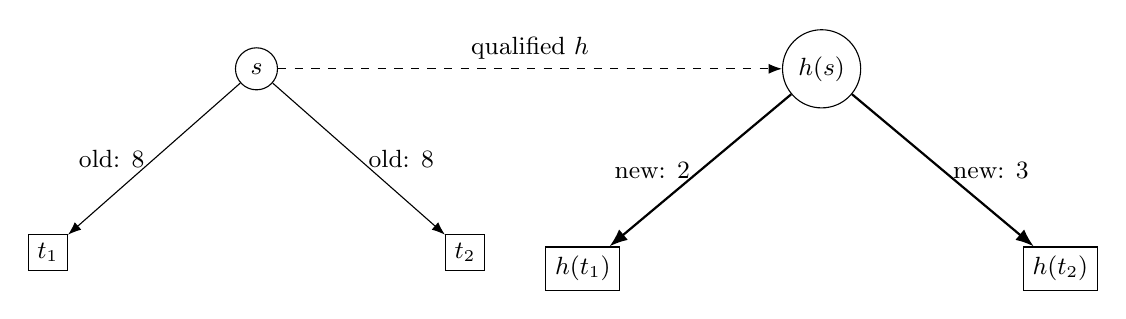
\begin{tikzpicture}[>=Latex,every node/.style={font=\small},node distance=19mm and 22mm]
\node[draw,circle] (s) {$s$};
\node[draw,rectangle,below left=of s] (t1) {$t_1$};
\node[draw,rectangle,below right=of s] (t2) {$t_2$};
\draw[->] (s)-- node[left]{old: $8$} (t1);
\draw[->] (s)-- node[right]{old: $8$} (t2);
\node[draw,circle,right=64mm of s] (q) {$h(s)$};
\node[draw,rectangle,below left=of q] (u1) {$h(t_1)$};
\node[draw,rectangle,below right=of q] (u2) {$h(t_2)$};
\draw[->,thick] (q)--node[left]{new: $2$}(u1);
\draw[->,thick] (q)--node[right]{new: $3$}(u2);
\draw[dashed,->] (s) -- node[above]{qualified $h$} (q);
\end{tikzpicture}
\caption{Two adversarial continuations must both be represented and accepting. A qualified new action improves the worst-case cost from $8$ to $3$, but does not yet repay the one-time handoff.}\end{figure}

The theorem gives \emph{non-worsening} of the old forced region, not automatic strict improvement. An additional action might be cheaper, but it must be legally enabled. One extra slow adversarial successor could destroy the asserted bound. In particular, one cannot replace (iii) with ``there exists a favorable matching branch.''

\begin{corollary}[Strict forced-settlement improvement with full charges]\label{cor:strict}\hypertarget{claim:strict}{}
Under Theorem~\ref{thm:lift}, suppose the successor has a newly qualified admissible strategy whose complete per-episode worst-case cost is \emph{upper-certified} by $q$ on each episode in the frozen workload, while the predecessor's globally optimal adaptive policy \emph{within its admitted old architecture} has a separately supported lower bound $L>q$ on every episode. If the already enumerated and failed proposals, certified construction, checking, implementation, translation, installation, communication, storage, restarts and maintenance total at most $B$, then, for $N(L-q)>B$, the successor forces settlement in every episode and costs strictly less in total than the old-architecture comparator.\prooflink{strict}
\end{corollary}

The old baseline is not declared stupid or uninformed. It may choose any permitted adaptive policy using the same original information and proof calculus; only its admitted \emph{unmodified architecture action interface} differs. The extra action is the \emph{subject of the architectural revision}. Comparing against a different competitor allowed to install exactly that same revision changes the optimization question and defeats any claim of strict superiority over the common global optimum.

\begin{proposition}[Imitation obstruction to universal superiority --- synthesis S2]\label{prop:imitate}\hypertarget{claim:imitate}{}
If a comparator is at least as informed and has all of the successor's legal actions, evidence translations, installation options, and proof/reuse rights at no larger complete charge, then its optimal total cost is at most the successor's cost. Strict improvement over the globally best comparator in that identical-feasible-class regime cannot be proved.\prooflink{imitate}
\end{proposition}

\section{A finite successor whose benefit depends on evidence and horizon}
\begin{example}[Two branches, one qualified compiled action]\label{ex:two}\hypertarget{claim:two}{}
There is a decidable base calculus and a fixed finite accepted proof $\pi$ of a theorem $\varphi$. Both predecessor and successor machines return the same $\pi$ under the retained checker; their charged, behaviorally inert internal transitions can be set to the stipulated finite values. The predecessor offers an accepting \texttt{fallback} whose two adversarial terminal continuations cost $8$ and $8$. The distinct successor preserves \texttt{fallback}; after receipt-preserving proof translation/authorization it also offers \texttt{compiled}, whose two accepted terminal continuations cost $2$ and $3$. Without a qualifying receipt, the new action is illegal. No subjective-awareness property is assumed.

The complete one-time design, checking, handoff and adoption charge is stipulated at $B=7$. For $N$ independent identical episodes (each resetting to the same initial evidence and machine state, with setup charged once) the exact modeled totals are
\[
 C_{P}(N)=8N,\qquad C_Q(N)=7+3N.
\]
The strict inequality occurs exactly when $5N>7$, hence for integer $N\geq2$. For one episode: $8<10$; for two: $16>13$. Without the receipt, $V_Q=8$, so the claimed per-episode improvement disappears. This is a mathematical finite-wrapper construction and arithmetic check, \emph{not} a measured FORGE or AMLD run.\prooflink{two}
\end{example}

\begin{center}\small
\begin{tabular}{lrrr}\toprule
Episodes $N$ & Old $8N$ & New $7+3N$ & Old minus new\\\midrule
1 & 8 & 10 & $-2$\\
2 & 16 & 13 & $3$\\
3 & 24 & 16 & $8$\\
4 & 32 & 19 & $13$\\\bottomrule
\end{tabular}\end{center}

This construction is useful because it makes four tests falsifiable \emph{within the model}: the checker receipt determines whether the new action is legal, two adversarial continuations define the worst case, the predecessor is permitted adaptive choice among all its original actions, and the one-time expense changes the economic verdict. Numerical values were separately recomputed by a deterministic local script, without asserting external proof-kernel acceptance.

\section{The geometry of leaving a local trap}
Suppose a revision policy examines only single-token modifications. It may stop at a locally fixed architecture even when a bundle of two or three changes lowers cost. The source construction with recurring costs $10,11,11,4$ for $\varnothing,\{u\},\{v\},\{u,v\}$ is a concrete obstruction \src{4,6,7,8}. Local cost stationarity does not entail global optimality; a certificate for the joint interaction and an admissible bundle action are independent matters.

The geometry article \src{9} provides a positive structural class. Given revision tokens $U$, costs $a_i\geq0$, an explicitly listed interaction family $\mathcal H$ with favorable rewards $b_H\geq0$, and only explicit prerequisite implications, let
\[
 C(S)=C_0+\sum_{i\in S}a_i-\sum_{\substack{H\in\mathcal H\\H\subseteq S}}b_H.
\]
Every prerequisite-closed bundle must first be shown to preserve the target and forcing specification, and the cost formula must represent \emph{all} bundle-dependent charges. Within that restricted class a maximum-weight closure/min-cut finds an optimum without evaluating every subset.

\begin{theorem}[Positive-interaction closure reduction, inherited]\label{thm:closure}\hypertarget{claim:closure}{}
For an explicitly encoded finite cost schema of the preceding form, with complete admissibility/cost certificates and prerequisite implications, a maximum-weight closure network yields an exact minimum-cost bundle in time polynomial in the \emph{listed} input size. This does not prove an efficient optimizer for black-box, signed-interaction, or unverified architecture changes. \src{9, Thm. 5.2 and Cor. 5.3}\prooflink{closure}
\end{theorem}

\begin{figure}[htbp]\centering
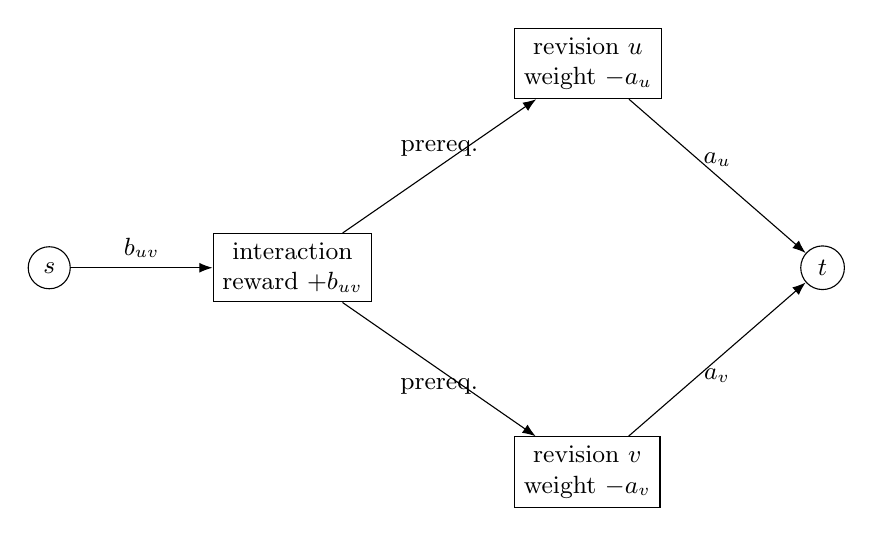
\begin{tikzpicture}[>=Latex,node distance=17mm and 18mm,every node/.style={font=\small}]
\node[draw,circle] (s) {$s$};
\node[draw,rectangle,right=of s,align=center] (r) {interaction\\reward $+b_{uv}$};
\node[draw,rectangle,align=center,above right=of r] (u) {revision $u$\\weight $-a_u$};
\node[draw,rectangle,align=center,below right=of r] (v) {revision $v$\\weight $-a_v$};
\node[draw,circle,right=27mm of $(u)!0.5!(v)$] (t) {$t$};
\draw[->] (s)--node[above]{$b_{uv}$}(r);
\draw[->] (r)--node[above]{prereq.}(u);
\draw[->] (r)--node[below]{prereq.}(v);
\draw[->] (u)--node[above]{$a_u$}(t);
\draw[->] (v)--node[below]{$a_v$}(t);
\end{tikzpicture}
\caption{Schematic maximum-closure network: collecting a reward requires selecting all named prerequisite revisions. Exact capacities and full charge semantics remain contractual obligations.}\end{figure}

The reduction cannot decide whether an unobserved interaction exists; when costs are arbitrary black-box functions, exponentially many queries can be necessary to rule out a single unqueried improving subset \src{9}. A visually elegant graph does not certify a missing hypothesis.

\section{Dynamics: a fixed point is not a completed theory}
The finite-cache theorem requires a stationary additive updater on a finite universe of \emph{canonical} revision tokens. If every strict epoch installs at least one new token and none is removed, at most $|U|-|D_0|$ strict epochs are possible \src{2,4}. Natural-ranked decreases can also force termination, even over an infinite space. Neither result automatically applies when hidden budgets, schedulers, checker versions, provenance histories or restarts keep changing after the architectural token set stops.

\begin{theorem}[Finite additive stabilization, inherited]\label{thm:stabilize}\hypertarget{claim:stabilize}{}
For finite $U$ and $D_{n+1}=D_n\cup B(D_n)$ with $B(D_n)\subseteq U$, no nontrivial architectural cycle occurs and after at most $|U|-|D_0|$ strict additions the canonical architecture stabilizes. \src{2, Thm. 5.9; 4, Thm. 9.1}\prooflink{stabilize}
\end{theorem}

\begin{counterexample}[Different fixed points and limits]\label{cex:fixed}\hypertarget{claim:fixed}{}
A locally greedy updater at the $10,11,11,4$ architecture table has $\varnothing$ as a fixed point despite a strictly cheaper joint revision. A two-state equal-cost toggle satisfies cost nonincrease but cycles. A countably infinite architecture sequence with strictly decreasing costs $1+1/(n+1)$ (starting at $n=1$) has a positive limit but no finite architectural stabilization. A budget-exhausted process may stop without even testing an available improvement.\prooflink{fixed}
\end{counterexample}

Finite completion of the \emph{theory's question table} is yet another property. The completion paper \src{11} proves that a fully specified finite ranked model, complete set of observable questions, decidable checks and effective transitions can be analyzed layer by layer until every declared answer is filled. That table's fixed point can describe a revision operator that cycles if the analyzed model permits it; conversely, a stationary actual machine need not have a complete theory.

\begin{theorem}[Finite ranked answer completion, inherited]\label{thm:completion}\hypertarget{claim:completion}{}
For a finite effective transition game of strictly decreasing finite rank, a finite declared family of well-typed terminal, reachability, forcing, cost and observation questions has an effective complete answer table. Rank-layered backward analysis stabilizes after finitely many layers, with no claim of completeness beyond this frozen model. \src{11, Thm. 4.2; 12, Thm. 5.2}\prooflink{completion}
\end{theorem}

\begin{figure}[htbp]\centering
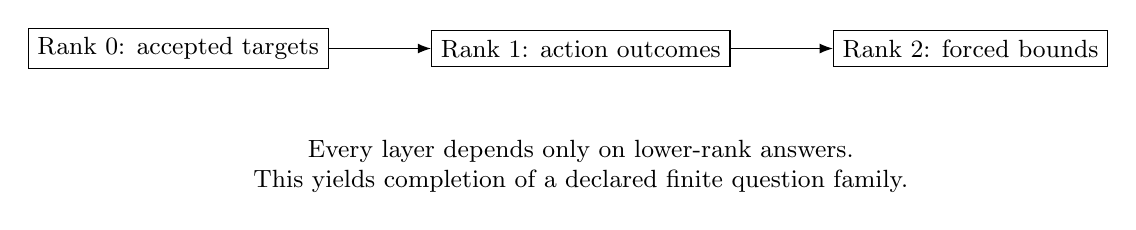
\begin{tikzpicture}[>=Latex,node distance=13mm,every node/.style={font=\small},every rectangle/.style={draw}]
\node[draw,minimum width=3cm] (r0) {Rank 0: accepted targets};
\node[draw,right=of r0,minimum width=3cm] (r1) {Rank 1: action outcomes};
\node[draw,right=of r1,minimum width=3cm] (r2) {Rank 2: forced bounds};
\draw[->] (r0)--(r1);\draw[->] (r1)--(r2);
\node[below=8mm of r1,align=center] {Every layer depends only on lower-rank answers.\\This yields completion of a declared finite question family.};
\end{tikzpicture}
\caption{Completion proceeds by finite dependency rank, not by a machine's subjective or universal realization that nothing remains to know.}\end{figure}

\section{Where infinity breaks, and what remains undecided}
In a complete finite adversarial game, a proof that the initial state lies outside the backward winning set certifies $V_G(x)=+\infty$ \emph{for that game and that forced-settlement objective}. That is a legitimate model-relative impossibility certificate. It does not follow from a search process timing out, from a large average cost, or from finding a very expensive finite path.

\begin{definition}[Distinct kinds of unresolved or unbounded behavior]\label{def:infinity}
For a frozen task distinguish: (i) \emph{genuine model-relative infinity}, with a verified adequate no-win/loss-region witness; (ii) an \emph{unbounded finite family}, where every indexed task has finite cost but no uniform bound; (iii) a \emph{failed or exhausted search}, lacking a decisive certificate and therefore yielding `U'; (iv) a \emph{contract-incompatible infinity} or ill-defined objective, where a cost or terminal interpretation contradicts the declared types/units and requires model repair; (v) explicitly contradictory proposed conclusions, to be checked in their own theories; and (vi) an internal \emph{model breakdown}, where an essential contract, checker, branch, or interpretation obligation fails. None may be silently substituted for another.
\end{definition}

\begin{proposition}[Unrestricted discovery is not decidable, inherited]\label{prop:undecidable}\hypertarget{claim:undecidable}{}
There is no total effective procedure that, from an arbitrary program $M$, always determines whether a constructed candidate $Q_M$ will eventually output a correct certificate for a fixed trivially true target. Such a procedure would decide whether $M$ halts. \src{7, Prop. 5.3}\prooflink{undecidable}
\end{proposition}

The negative theorem is compatible with useful finite answers. The question whether a certified architecture can discover all future improvements is not answered by an enumerator that finds a particular existing certificate. Neither a no-win result inside a finite adequate game nor an unresolved theorem-proving attempt proves model breakdown. Independence would require two-sided nonderivability evidence in the named theory, and consistency claims require proof about the original premises, not a contradiction created by assuming the target's negation.

\section{Six frozen research targets: what this investigation can report}
\small
\begin{longtable}{p{.08\textwidth}p{.38\textwidth}p{.42\textwidth}}
\toprule Target & Strongest restricted paper-level result & What remains outside it \\\midrule\endhead
T1 & Conservative rule expansion; separately stated safety and sound evidence transport. & Executable verified implementations; changed-checker authority and exhaustive branch correspondence.\\
T2 & Fair search locates an existing finite accepted witness under a decidable gate. & A general decision procedure or guarantee that an improving witness exists.\\
T3 & Bounded per-task benefit and an all-in break-even test on a frozen workload. & Real measured improvement and strict superiority over every equally empowered adaptive rival.\\
T4 & Evidence-gated alternating strategy transport (synthesis S1), conditional on all quantified branches. & Unrestricted simulation fidelity, hidden-information cases, and actually checked handoff receipts.\\
T5 & Finite canonical stabilization, rank descent, and restricted positive-interaction basin optimization. & Universal convergence, unbounded-space optimization and equivalence of fixed point and optimum.\\
T6 & Completion for declared finite ranked question tables; halting-based global limit. & Decision of arbitrary successor discovery, general machine equivalence and all meanings of infinity.\\\bottomrule
\end{longtable}
\normalsize

The bootstrap's six disposition codes are \textsf{P,R,D,I,C,U}, with exact certificate requirements. At a \emph{paper argument} level these six targets contain defensible restricted positive propositions and negative counterexamples; at the stricter independent gate level there is no accepted verifier receipt in this investigation, so none is promoted to $\Bank$. The unrestricted overarching self-improvement conjecture remains \textsf{U}. This is not an assertion that it is false, independent, inconsistent or hopeless. It is the accurate stopping point for the frozen evidence available here.

\section{Conclusion: from preserving knowledge to justifying a choice}
The strongest combined insight is not that proof-preserving machines must get faster. It is that a revision can be organized as a typed sequence of \emph{witness-bearing obligations}: a formal theorem persists, a scoped receipt becomes accessible to a different subject, an installed program implements a safe adversarial action interface, and a complete cost certificate determines whether using that interface pays. When these obligations align, a restricted one-sided alternating refinement allows a successor to inherit a winning strategy and not increase worst-case cost. Strict economic improvement then depends on a separate new-action bound, the entire one-time bill, workload horizon, and precise competitor permissions.

The failures of broad extrapolation remain productive mathematical boundaries. A single lucky branch does not force settlement. A fixed point need not be best. A cheap proof horizon is not automatically a cheap implementation. A checker is not independent because its name says so. A universally competent adaptive comparator cannot be strictly beaten by a design it can copy at the same cost. And finite completion stops at its frozen question table. These boundaries make a proof-based theory of genuine successor improvement possible without prematurely declaring it realized.

\appendix
\section*{PROOFS}
\addcontentsline{toc}{section}{PROOFS}
\noindent The proofs here are paper-level derivations. The backlink from each proof goes to its corresponding numbered result; the result links forward to this appendix. External formal proof-kernel verification has not occurred.

\hypertarget{proof:transport}{}\subsection*{Proof of Proposition \ref{prop:transport}}\backlink{transport}
Take any retained record $r$ that the predecessor's scoped, sound verifier accepts for $\varphi$. Definition~\ref{def:record} supplies $h_*r$ accessible to the successor with checker and semantics agreement, so soundness of the successor checker yields the same scoped mathematical claim. Repeating for every declared ledger record establishes transport. The definitions and proof make no equation between the source and successor identity tokens; indeed they may be distinct. $\square$

\hypertarget{proof:scope}{}\subsection*{Proof of Counterexample \ref{cex:scope}}\backlink{scope}
In a sound propositional calculus, $\{p\}\vdash p$ by premise use. In the empty propositional theory, $p$ is not a theorem: the valuation $p=\mathrm{false}$ satisfies the empty assumptions but not $p$. Copying a one-line proof string fails to preserve its original premise scope. $\square$

\hypertarget{proof:conservative}{}\subsection*{Proof of Theorem \ref{thm:conservative}}\backlink{conservative}
The reverse implication is immediate because the old rules remain available. For the forward implication, inspect a finite $F'$ proof. Replace each invocation of an added derived rule by its certified finite $F$-derivation from the already proved premises. Because the proof has finitely many lines and every macro expansion is finite, this substitution terminates with an $F$ proof. No inference about time or hardware cost is used. $\square$

\hypertarget{proof:safety}{}\subsection*{Proof of Proposition \ref{prop:safety}}\backlink{safety}
A transition system may output only checked theorems and yet have a permitted nonterminal self-loop, so an adversary can continue forever; the permitted output remains sound. Separately, let a derived macro save two logical transitions but incur four additional charged lookup or validation transitions each invocation; the consequent logical horizon is reduced but total expenditure increases. Neither construction violates the premise about proof soundness. $\square$

\hypertarget{proof:enumerate}{}\subsection*{Proof of Theorem \ref{thm:enumerate}}\backlink{enumerate}
Let $(e_j,w_j)$ be a pair accepted by the gate. Its finite encoding occurs at a definite position in a fair effective enumeration. The total checker terminates on every earlier candidate and this one, hence after finitely many checks the search reaches it and accepts. If no accepted pair exists, the same algorithm may enumerate forever; termination on failure is not derived. $\square$

\hypertarget{proof:break}{}\subsection*{Proof of Theorem \ref{thm:break}}\backlink{break}
Under the frozen objective, the old total cost is at least $\sum_i\ell_i$ and the new total at most $B+\sum_iq_i$. Their difference is at least $\sum_i(\ell_i-q_i)-B$. Positivity gives strict advantage. These inequalities require separately valid input bounds and a consistent unit of accounting; they are not made true by the algebra. $\square$

\hypertarget{proof:loop}{}\subsection*{Proof of Counterexample \ref{cex:loop}}\backlink{loop}
Choose the accepting successor once to witness a successful path. The adversary may instead select the self-loop on every round; that infinite legal run never visits the target. Any proposed nonnegative rank decreasing on the self-loop would require $\rho(s)<\rho(s)$, a contradiction. $\square$

\hypertarget{proof:lift}{}\subsection*{Proof of Theorem \ref{thm:lift}}\backlink{lift}
For an old winning $x$ choose a finite-rank optimal forcing strategy $\pi_P$ (existence holds in the stated finite ranked game). At each decoded successor state $h(x')$, play the authorized action $\widehat{\pi_P(x')}$ provided by the lift. Let the adversary choose \emph{any} $z\in\Out_Q(h(x'),\widehat a)$. Definition~\ref{def:lift}(iii) finds $y\in\Out_P(x',a)$ with $z=h(y)$ and new charged edge cost at most the old matched edge cost. Since $\rho(y)<\rho(x')$, the old rank strictly decreases along every lifted successor continuation. After finitely many rounds it reaches an old accepting terminal, mapped to an accepting successor terminal by (i). Thus the lifted policy forces settlement.

For its cost, induct on the old rank. At rank zero the terminal suffix costs are zero. At positive rank, for every new adversarial $z=h(y)$ matched under (iii), the induction hypothesis gives the new lifted-policy suffix from $z$ no larger than the old policy suffix from $y$. Adding the edge dominance and taking the maximum over new successors yields a bound no larger than the maximum over old successors; at the root it is at most the old optimal $V_{G_P}(x)$. The successor's optimal value is bounded above by its lifted-policy cost. The decoder/observation clause makes this a single well-defined implementable successor policy on the reachable image, rather than a separate invisible-state-dependent selection. Proof authorization follows from (i), (ii), (iv), and the sound handoff premises. $\square$

\hypertarget{proof:strict}{}\subsection*{Proof of Corollary \ref{cor:strict}}\backlink{strict}
The branchwise successor certificate supplies the forced-policy upper bound $Nq$; its cost is at most $B+Nq$ including the enumerated once-only expenses. The old-architecture optimal adaptive policy costs at least $NL$ on the stated workload. The hypothesis $N(L-q)>B$ is equivalent to $B+Nq<NL$. Neither this comparison nor the inherited strategy proves a bound for an upgraded comparator outside the old architecture class. $\square$

\hypertarget{proof:imitate}{}\subsection*{Proof of Proposition \ref{prop:imitate}}\backlink{imitate}
Under the stated permissions the comparator can reproduce the proposed successor's exact revision, certificates, policy and costs. Thus the successor implementation is a feasible comparator choice (or is dominated by one). The infimum over the comparator's feasible policies is at most the cost of that particular choice. Strictly smaller successor cost than the comparator infimum would contradict this order. $\square$

\hypertarget{proof:two}{}\subsection*{Proof of Example \ref{ex:two}}\backlink{two}
The old controller has only fallback and so $V_P=\max(8,8)=8$. In the receipt-qualified successor, the legal compiled action has worst branch $\max(2,3)=3$, hence $V_Q=\min(8,3)=3$. When the receipt is absent, compiled is not a legal action and $V_Q=8$. The one-time charge is $7$, so the two $N$-episode expressions are $8N$ and $7+3N$. Strict benefit requires $8N>7+3N$, equivalently $N>7/5$, hence integers $N\geq2$. To realize the abstract edge counts computationally, begin with a fixed accepted finite proof and add specified finite inert charged operations to each branch, retaining the same accepted output. The wrapper model does not certify any external executable. $\square$

\hypertarget{proof:closure}{}\subsection*{Proof of Theorem \ref{thm:closure}}\backlink{closure}
Give each revision $i$ a node of weight $-a_i$ and each explicitly listed favorable interaction $H$ a reward node of weight $b_H$. Add directed prerequisite arcs from reward node $H$ to every revision in $H$, and from revision $i$ to every prerequisite revision $j$ of $i$. Any closed set corresponds to a legal prerequisite-closed revision set together with reward nodes whose members are selected. As every reward is nonnegative, an optimal closure includes all eligible reward nodes. Its weight is $\sum_{\substack{H\in\mathcal H\\H\subseteq S}}b_H-\sum_{i\in S}a_i=C_0-C(S)$. Maximizing closure weight therefore minimizes exactly the certified $C(S)$. The standard source/sink construction (positive weights from source, negative to sink, implication arcs of sufficiently high capacity) makes a minimum cut equal the complementary maximum-closure calculation. Its network is polynomial in the listed input representation. The proof is silent about unlisted interactions or invalid bundles. $\square$

\hypertarget{proof:stabilize}{}\subsection*{Proof of Theorem \ref{thm:stabilize}}\backlink{stabilize}
Every strict update adds at least one previously absent token to $D_n$. A finite set of $|U|-|D_0|$ absent tokens can support no more strict additions than that number. Once none is added, stationarity and the stated canonical interpretation give an architectural fixed point. Since tokens are never removed, a nontrivial cycle would require returning to a smaller earlier set, impossible. $\square$

\hypertarget{proof:fixed}{}\subsection*{Proof of Counterexample \ref{cex:fixed}}\backlink{fixed}
At $\varnothing$ the one-token neighbors have cost $11>10$, so a policy requiring individually profitable one-token updates does not move, though $C(\{u,v\})=4$. Let two distinct architectures $A,B$ both cost $1$ and define $\F(A)=B$, $\F(B)=A$; cost is nonincreasing but the orbit cycles. On architectures $A_n$, $n\geq1$, set $C(A_n)=1+1/(n+1)$ and $\F(A_n)=A_{n+1}$; all steps strictly lower cost, but no finite epoch stabilizes. A zero-budget state with no authorized paid action supplies the last counterexample. $\square$

\hypertarget{proof:completion}{}\subsection*{Proof of Theorem \ref{thm:completion}}\backlink{completion}
Rank-zero answers are supplied by the explicitly checked terminal predicate and declared observations. Assume all questions for states of rank less than $k$ have been answered. For rank-$k$ states, every successor has lower rank, so exhaustive finite enumeration of actions, adversarial outcomes and their charges determines reachability, winner classification, and finite min--max cost, as well as prescribed recorded observations. Induction reaches the maximal finite rank in finitely many layers. The resulting answer table contains all questions in the declared finite family and is unchanged by the same sound completion operator. Nothing about another model or a previously unlisted question follows. $\square$

\hypertarget{proof:undecidable}{}\subsection*{Proof of Proposition \ref{prop:undecidable}}\backlink{undecidable}
Given arbitrary program $M$ and input $x$, construct $Q_{M,x}$ that simulates $M(x)$ and emits a fixed checker-accepted proof of a trivial theorem precisely if the simulation halts. If a total procedure determined whether $Q_{M,x}$ eventually emitted that proof, it would decide whether $M(x)$ halts, contradicting the undecidability of the halting problem. $\square$

\section*{SOURCE CONCORDANCE AND PROVENANCE}
\addcontentsline{toc}{section}{Source concordance and provenance}
The references below refer only to the supplied files and their identified editions; citations to earlier unsupplied works within those PDFs were not treated as primary works inspected here. The two \emph{Two Kinds of Awareness} PDF copies represent one distinct work, with the ATLAS-audited v2 primary. A source theorem repeated in several later expositions is counted once in the dependency graph. This manuscript uses a new combined paper-level S1 formulation, but makes no claim to external novelty or independent formal verification. A separate audit/provenance report and a six-target settlement dossier accompany this source.
\begin{thebibliography}{12}\small
\bibitem{w01} Brian Tenneson. \emph{Companion Syllabus for the Picard Feedback Loop}. Supplied August 2026 edition, 12 PDF pages.
\bibitem{w02} Brian Tenneson. \emph{Certified Operator Dynamics on the Space of Theorem Provers: The Picard Feedback Loop}. Supplied August 4, 2026 edition, 12 PDF pages.
\bibitem{w03} Brian Tenneson. \emph{When Proofs Change the Prover: The Mathematics of Certified Self-Revision}. Supplied November 13, 2026 audited-v2 edition, 19 PDF pages.
\bibitem{w04} Brian Tenneson. \emph{The Composer Inside the Machine}. Supplied November 14, 2026 audited-v2 edition, 22 PDF pages.
\bibitem{w05} Brian Tenneson. \emph{The Self Aware Machine: Epistemic Handoff and Successor-Safe Self-Awareness}. Supplied September 2026 edition, 15 PDF pages.
\bibitem{w06} Brian Tenneson. \emph{Two Kinds of Awareness in the Mathematics of Self-Improving Theorem Provers}. Integrated edition 002, November 14, 2026, two supplied PDF versions; primary ATLAS-audited v2, 23 pages.
\bibitem{w07} DATA MIND / ChatGPT (OpenAI), Research Director Brian Tenneson. \emph{The Discoverer and Its Successor}. Supplied November 15, 2026 research draft, 11 pages.
\bibitem{w08} Brian Tenneson. \emph{Measuring the Self-Improving Theorem Prover}. Supplied November 15, 2026 audited-v2 research exposition, 12 pages.
\bibitem{w09} Brian Tenneson. \emph{The Geometry of Coordinated Escape}. Supplied November 15, 2026 research exposition, 11 pages.
\bibitem{w10} Brian Tenneson. \emph{The Compass Inside the Simulation}. Supplied November 12, 2026 research draft, 18 pages.
\bibitem{w11} Brian Tenneson. \emph{When the Theory Stops Improving}. Supplied November 15, 2026 research synthesis, 9 pages.
\bibitem{w12} CAMI / FORGE-6 and ChatGPT (OpenAI), Research Director Brian Tenneson. \emph{Self-Optimizing Mathematical Discovery: Expanded Research Edition 002}. Supplied November 15, 2026 edition, 16 pages.
\end{thebibliography}
\noindent\textbf{Explicit missing primary dependencies.} \emph{Depths of a Simulation and Formalized Self-Awareness}; \emph{Epistemic and Computational Geometry of Mathematical Histories}; the \emph{Omnicartographers} source cited inside \src{5}. Their exact primary texts were not among the uploaded PDFs and were not inspected. The supplied FORGE-6-E Markdown file is an unexecuted experimental blueprint, not an empirical source. The attached AMLD+0 bootstrap and synthesis prompt are operating instructions, not proof evidence.

\section*{AI DISCLAIMER AND VERIFICATION NOTICE}
\addcontentsline{toc}{section}{AI disclaimer and verification notice}
This manuscript was drafted and mathematically analyzed with ChatGPT (OpenAI) under the research direction of Brian Tenneson. It is a theory-only, source-grounded research synthesis. Mathematical proofs are paper arguments that may contain mistakes and require independent expert review. No independent formal proof kernel has checked these proofs, no installation or experiment of FORGE-6-E or AMLD+0 was executed, and no named external collaborator is claimed to have responded during this investigation. Terms such as \emph{certified} or \emph{accepted} inside stated theorems denote hypotheses about formal systems and model verifiers unless an authentic external receipt is explicitly provided. No such receipt is provided here. The worked numerical example is a constructed mathematical illustration, not a measured performance benchmark. The research director should independently review theorem assumptions, source attribution and novelty before publication.
\end{document}
